% master.tex : master-fil for projektet
% ------------------------------------------------------------------------------
% Dette er hovedfilen for projektet, hvori indhold fra alle input-filer (tekst,
% billeder, litteraturdatabaser, osv.) samles

% Dokumenttypen 'book' er valgt pga. dens mange fleksible indstillinger
% Se https://tex.stackexchange.com/a/36989/118167
\documentclass[11pt,a4paper,twoside,openright,danish]{book}

% Variabler, som bruges til automatisk at indsætte titel, forfattere, osv. på
% forsiden og titelbladet.
\def \projecttitle       {P1-projekt 2020 for matematik-økonomi}
\def \projectsubtitle    {Optimering af gaslager}
\def \projecttheme       {Optimering af gaslager}
\def \projectdegree      {Matematik-Økonomi}  % eller Matematik-Økonomi/Teknologi
\def \projectperiod      {Efterårssemesteret 2020}
\def \projectnumber      {P1}
\def \projectgroup       {B350}
\def \projectauthors     {
  Beate Marcussen\\
  Marcus Søndergaard Aaskoven\\
  Mathias Graversen\\
  Mattias Adam Arvidsson\\
  Vennan Vithiyatharan
  % ...
}
\def \projectsupervisors {
  PJanus Valberg-Madsen\\
  % ...
}

% Preamblet indeholder alle de indstillinger og makroer, som skal indsættes for
% hovedindholdet, og i denne skabelon samles det i filen aaumath.sty, som
% definerer en pakke, der kan indlæses med \usepackage.
\usepackage{aaumath}
\usepackage{graphicx}
% Dokumentets indhold indsættes mellem \begin- og \end-makroerne for
% 'document'-blokken
\usepackage{amsthm}
\theoremstyle{definition}
\newtheorem{definition}
{Definition}[section]

\begin{document}

% Dokumentets 'front matter' tælles ikke med ifm. antal sider og nummereres med
% romerske tal. Herunder hører f.eks. forsiden, titelbladet, forordet og
% indholdsfortegnelsen.
\frontmatter
% incl/misc/frontpage.tex : rapportens forside
% ------------------------------------------------------------------------------


\backgroundsetup{
  scale = 1,
  angle=0,
  opacity=1,
  contents = {
    
\includegraphics[width=\paperwidth,height=\paperheight]{fig/img/aau/waves.pdf}
  }
}
\BgThispage
\pdfbookmark[0]{Forside}{forside}
\begin{titlepage}
  \centering
  \phantom{}
  \vspace{2cm}

  % AAU-segl
  \begin{minipage}[c]{0.2\paperwidth}
    \centering
    \makebox[0pt]{
      % fig/tikz/aau-badge.tex : AAU-logo til forsiden
% ------------------------------------------------------------------------------

\begin{tikzpicture}
  % Tegn hvid cirkel og tilføj det gennemsigtige, blå logo ovenpå
  \node[circle,color=white,fill=white,minimum size=1.175\textwidth] at (0,0) {};
  \node at (0,0) {
\includegraphics[width=\textwidth]{fig/img/aau/logo-circle.pdf}};
\end{tikzpicture}

    }
  \end{minipage}

  % Hovedindhold
  \vspace{4cm}
  {\fontfamily{bch}\selectfont
    \fboxsep0pt\colorbox{white}{
      \begin{minipage}{\textwidth}
        \centering
        \color{AAUblue1}

        \vspace{2em}
        {\Huge\bfseries\projecttitle}

        {\Large\bfseries\projectsubtitle}

        \bigskip
        \parbox{\textwidth}{\centering\large\projectauthors}

        \bigskip
        {\bfseries\large{\projectnumber}-Projekt, Gruppe \projectgroup, \projectdegree}
        \vspace{2em}
      \end{minipage}
    }
  }

\end{titlepage}

% incl/misc/titlepage.tex : rapportens titelblad
% ------------------------------------------------------------------------------
% Titelbladet genereres af makroen \aautitlepage, som er defineret i
% /incl/pre/ext/aautitlepage.sty


\pdfbookmark[0]{Titelblad}{titelblad}
\aautitlepage{
  \projectinfo{
    \projecttitle
  }{
    \projecttheme
  }{
    \projectperiod
  }{
    Gruppe \projectgroup
  }{
    \parbox[t]{\textwidth}{\projectauthors}
  }{
    \parbox[t]{\textwidth}{\projectsupervisors}
  }{
    \today
  }
}{
  \textbf{Institut for Matematiske Fag}\\
  Skjernvej 4A\\
  DK-9220 Aalborg Ø\\
  \href{http://math.aau.dk}{http://math.aau.dk}
}{
  % incl/misc/abstract.tex : projektets abstract 

This study investigates how algorithms and graph theory can help with the optimization of profit from a gas storage, over the course of a given period of time, by buying and selling gas units. 

In order to give clarification of the calculations and methods used in this study, the essential and relevant graph theory, and theory of algorithms will therefore be explained.
During this study it was found that Dijkstra's algorithm was very useful for solving shortest path problems in graphs. This study implements Dijkstra's algorithm in Python 3 in order to find the longest path through a graph. This can be done by finding the shortest path through the inverted non-negative graph. This path will be the path that yields the greatest profit. In addition, this path is the one that will give us the most optimal trading strategy.

The greatest profit in the original problem is 252.73€, and in the extended problem, it is 188.27€. From this, it can be concluded that the extensions that have been made, significantly reduce the profit. This is mainly due to the fluctuating limits of inventory, and the limits of buying and selling per month, as they affect the profit over the course of several months, compared to the penalty factor which only affects the last two months.

}

\tableofcontents

% Dokumentets 'main matter' (hovedindhold) er der, hvor det meste indhold skal
% sættes ind. Sider og overskrifter er nummererede med arabiske tal.
\mainmatter

\chapter{Forord}
Følgende projekt er udarbejdet af gruppe B350 bestående af fem stud.scient.oeconer på 1. semester. Projektet er skrevet i efteråret 2020 og beskæftiger sig med diskret matematik herunder optimering af et gaslager som basisproblem. Diskret matematik indgår i studiets læreplan og er derfor et relevant emne til projektskrivning. Projektet er skrevet i \LaTeX, og delt via GitAhead.
%Vi vil som gruppe rette en stor tak til vores vejleder Janus Valberg-Madsen for godt samarbejde gennem projektforløbet samt gode råd og rettelser.

\chapter{Indledning}

\chapter{Grafteori}
Følgende kaptel er skrevet med afsæt i [Rosen, kaitel 10].

Grafer er diskrete strukturer bestående af et antal punkter, også betegnet knuder, samt et antal kanter, der forbinder disse knuder. Punkterne illustreres ofte som prikker, mens kanterne repræsenteres af streger eller pile, der forbinder disse prikker. Graferne varierer alt efter deres type og funktion, og de mange forskellige egenskaber betyder, at problemer i næsten enhver tænkelig disciplin kan løses ved hjælp af grafmodeller. Vi vil eksempelvis i dette projekt benytte grafteori og princippet om den korteste vej til at optimere et gaslager.
\section{Graftyper}
En graf er som nævnt tidligere nævnt en struktur med punkter og kanter. Den er givet ved definitionen:
\begin{definition}
[Graf] 
En graf $G=(V,E)$ består af $V$, et sæt punkter(knuder), hvor $V\neq0$, og et sæt kanter, $E$. Hver kant forbinder én eller to punkter kaldet dets endepunkter.
\end{definition}
Det fremgår af definitionen, at en graf ikke kan have 0 punkter, men en lignende afgrænsning i den anden ende eksisterer ikke. Der kan altså godt være uendeligt mange knuder og kanter. I så fald kaldes det en uendelig graf. Ellers kaldes det en endelig graf, og det er denne type, som vi beskæftiger os med i projektet.
Ydermere, ses det i definitionen at hver kant forbinder én eller to punkter. For en simpel graf gælder det, at ingen kanter forbinder et punkt med sig selv. Der må altså ikke være løkker. Derudover forbindes to punkter med max én kant.
\begin{figure}[H]
\centering
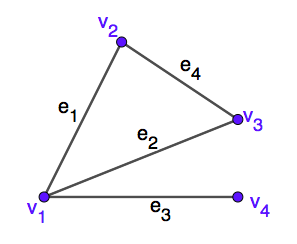
\includegraphics[scale=0.5]{simpel_graf.png}
\caption{En simpel graf}
\label{fig:simpel}
\end{figure}
I kontrast til den simple graf finder vi multi-grafen. For denne type graf skal der være flere kanter, der forbinder det samme sæt punkter. Der må stadig ikke optræde løkker.
\begin{figure}[H]
\centering
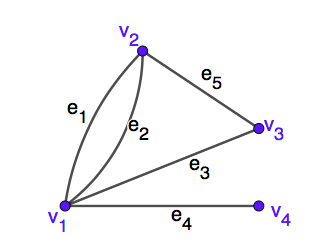
\includegraphics[scale=0.5]{multigraf.png} 
\caption{En multigraf}
\label{fig:multi}
\end{figure}
I eksemplet ovenover ses det, at to kanter forbinder punktsættet ($v_{1},v_{2}$). Hvis en graf, modsat de to allerede nævnte, kan indeholde både løkker og flere kanter der forbinder de samme punkter kaldes det en pseudo-graf. Vi ser i eksemplet herunder, at der er to kanter, der forbinder $v_{1}$ og $v_{2}$, og der er en løkke ved $v_{4}$.
\begin{figure}[H]
\centering
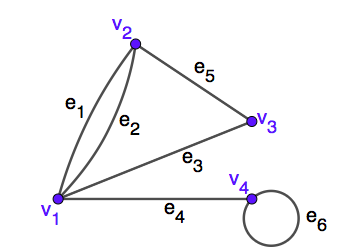
\includegraphics[scale=0.5]{pseudograf.png}
\caption{En pseudograf med et loop}
\label{fig:pseudo}
\end{figure}
En anden typisk grafopdeling er opdelingen i orienterede og ikke-orienterede grafer. For en orienteret graf gælder det, at dets kanter har en retning. Dette er ofte illustreret med pile. Den har dermed et startpunkt og et endepunkt. Disse grafer kan defineres ved:
\begin{definition}
[Orienteret graf] 
En orienteret graf $(V,E)$ består af $V$, et sæt punkter(knuder), hvor $V\neq0$, og et sæt orienterede kanter, $E$. Hver orienterede kant forbinder et sæt punkter $(u,v)$ startende i punktet $u$ og sluttende i punktet $v$.
\end{definition}
Der kan foruden disse to også være tale om mixede grafer, som er grafer med både orienterede og ikke-orienterede kanter. Vi vil i projektet beskæftige os med orienterede grafer, da det er denne type vi bruger til optimeringen af gaslageret. I vores tilfælde vil vi nemlig tildele kanterne vægt, som der beskrives i følgende afsnit


\section{Vægtede grafer}
Grafer med vægte tildelt deres kanter kan bruges til at løse problemer såsom at finde korteste vej mellem to byer i et transportnetværk. 

\section{Sektion 3}
\chapter{Analyse}
\section{Sektion 1}

\section{Sektion 2}

\section{Sektion 3}
\chapter{Vurdering af metoderne}
\section{Sektion 1}

\section{Sektion 2}

\section{Sektion 3}
\chapter{Konklusion}
%\chapter{Forord}
Følgende projekt er udarbejdet af gruppe B350 bestående af fem stud.scient.oeconer på 1. semester. Projektet er skrevet i efteråret 2020 og beskæftiger sig med diskret matematik herunder optimering af et gaslager som basisproblem. Diskret matematik indgår i studiets læreplan og er derfor et relevant emne til projektskrivning. Projektet er skrevet i \LaTeX, og delt via GitAhead.
%Vi vil som gruppe rette en stor tak til vores vejleder Janus Valberg-Madsen for godt samarbejde gennem projektforløbet samt gode råd og rettelser.







% Input-filer bør opdeles således, at hver fil svarer til et kapitel. Makroen
% \include indsætter et sideskift og indholdet fra den givne stil.

% \include{incl/main/example1}
% \include{incl/main/example2}
% ...

% Appendicer indsættes inde i en appendices-blok og bliver nummereret med
% bogstaver i stedet for tal
\begin{appendices}
  % \include{incl/app/appendix1}
  % \include{incl/app/appendix2}
  % ..
\end{appendices}

% Dokumentets 'back matter' er til ekstra ting som f.eks. litteraturlisten.
% Overskrifter bliver ikke nummereret her.
\backmatter

% Automatisk litteraturliste baseret på, hvilke kilder, der er blevet refereret
% til i løbet af rapporten.
\bibliographystyle{apalike}
\bibliography{
  incl/bib/books,
  incl/bib/articles,
  incl/bib/software
}

\end{document}
